%package list
\documentclass{article}
\usepackage[top=3cm, bottom=3cm, outer=3cm, inner=3cm]{geometry}
\usepackage{graphicx}
\usepackage{url}
\usepackage{multirow}
%\usepackage{cite}
\usepackage{hyperref}
\usepackage{array}
\usepackage{multicol}
\newcolumntype{x}[1]{>{\centering\arraybackslash\hspace{0pt}}p{#1}}
\usepackage{natbib}
\usepackage{pdfpages}
\usepackage{multirow}
\usepackage{float}
\usepackage[normalem]{ulem}
\useunder{\uline}{\ul}{}




%%%%%%%%%%%%%%%%%%%%%%%%%%%%%%%%%%%%%%%%%%%%%%%%%%%%%%%%%%%%%%%%%%%%%%%%%%%%
%%%%%%%%%%%%%%%%%%%%%%%%%%%%%%%%%%%%%%%%%%%%%%%%%%%%%%%%%%%%%%%%%%%%%%%%%%%%
\newcommand{\csemail}{vmachacaa@unsa.edu.pe}
\newcommand{\csdocente}{Vicente Machaca Arceda}
\newcommand{\cscurso}{Algoritmos y Estructura de Datos}
\newcommand{\csuniversidad}{Universidad Nacional de San Agustín}
\newcommand{\csescuela}{Maestría en Ciencia de la Computación}
\newcommand{\cspracnr}{Final}
\newcommand{\cstema}{--}
%%%%%%%%%%%%%%%%%%%%%%%%%%%%%%%%%%%%%%%%%%%%%%%%%%%%%%%%%%%%%%%%%%%%%%%%%%%%
%%%%%%%%%%%%%%%%%%%%%%%%%%%%%%%%%%%%%%%%%%%%%%%%%%%%%%%%%%%%%%%%%%%%%%%%%%%%


\usepackage[english,spanish]{babel}
\usepackage[utf8]{inputenc}
\AtBeginDocument{\selectlanguage{spanish}}
\renewcommand{\figurename}{Figura}
\renewcommand{\refname}{Referencias}
\renewcommand{\tablename}{Tabla} %esto no funciona cuando se usa babel
\AtBeginDocument{%
	\renewcommand\tablename{Tabla}
}

\usepackage{fancyhdr}
\pagestyle{fancy}
\fancyhf{}
\setlength{\headheight}{30pt}
\renewcommand{\headrulewidth}{1pt}
\renewcommand{\footrulewidth}{1pt}
\fancyhead[L]{\raisebox{-0.2\height}{
\includegraphics[width=3cm]{Img/logo_unsa.jpg}}}
\fancyhead[C]{}
\fancyhead[R]{\fontsize{7}{7}\selectfont	\csuniversidad \\ \csescuela \\ \textbf{\cscurso} }
\fancyfoot[L]{MSc. Vicente Machaca}
\fancyfoot[C]{\cscurso}
\fancyfoot[R]{Página \thepage}







\begin{document}
	
	\vspace*{10px}
	
	\begin{center}	
		\fontsize{17}{17} \textbf{ Proyecto \cspracnr}
	\end{center}
	%\centerline{\textbf{\underline{\Large Título: Informe de revisión del estado del arte}}}
	%\vspace*{0.5cm}
	

	\begin{table}[h]
		\begin{tabular}{|x{4.7cm}|x{4.8cm}|x{4.8cm}|}
			\hline 
			\textbf{DOCENTE} & \textbf{CARRERA}  & \textbf{CURSO}   \\
			\hline 
			\csdocente & \csescuela & \cscurso    \\
			\hline 
		\end{tabular}
	\end{table}	
	
	
	\begin{table}[h]
		\begin{tabular}{|x{4.7cm}|x{4.8cm}|x{4.8cm}|}
			\hline 
			\textbf{PRÁCTICA} & \textbf{TEMA}  & \textbf{DURACIÓN}   \\
			\hline 
			\cspracnr & Algoritmos de ordenamiento  & 3 horas   \\
			\hline 
		\end{tabular}
	\end{table}
	
	
	\section{Datos de los estudiantes}
	Grupo: N° 8
	\begin{itemize}
		\item Integrantes: 
		\begin{itemize}
			\item Esai Josue Huaman Meza
			\item Alan Jerry Reyes Robles
			\item Jorge Luis Zegarra Guardamino
			\item Nestor Giraldo Calcinas Huaranga
		\end{itemize}		
	\end{itemize}
	
	
	
	
	
	
	\section{Introducción}
	
	Este proyecto final trata de la detección de correos SPAM.

    Para esto se usará una parte del código utilizado en la práctica 04, para luego implementar un descriptor que para este caso será una bolsa de palabras.

    Para todo ello, el lenaguaje de programamción a usar será Java Script.

    Para todo ello, el lenaguaje de programamción a usar será Java Script.
	
El repositorio Github se encuentra en el siguiente enlace \href{https://github.com/nestorcal/kdtree}{Estructura KD-Tree}.
El video explicativo se encuentra en el siguiente enlace \href{https://drive.google.com/file/d/1SdcIBezyhSePjlnDmgkuoMWF9ytabTYo/view}{Algoritmo Multidimencional KD-Tree-Grupo8}.
	
	\section{Estructuras de Datos Multidimensional}\label{sec:ejercicios}
	\begin{enumerate}
		\item \textbf{Estructura de datos KD-Tree}
		
			La estructura KD-Tree es una estructura de datos de particionado del espacio que organiza los puntos en un Espacio euclídeo de k dimensiones.

La Estructura KD-Tree se puede construir de la siguiente manera: 

\begin{itemize}
   \item Conforme se desciende en el árbol, se emplean ciclos a través de los ejes para seleccionar los planos.
   \item En cada paso, el punto seleccionado para crear el plano de corte será la mediana de los puntos puestos en el árbol kd, lo que respeta sus coordenadas en el eje que está siendo usado.

\end{itemize}	

\begin{figure}[H]
\centering
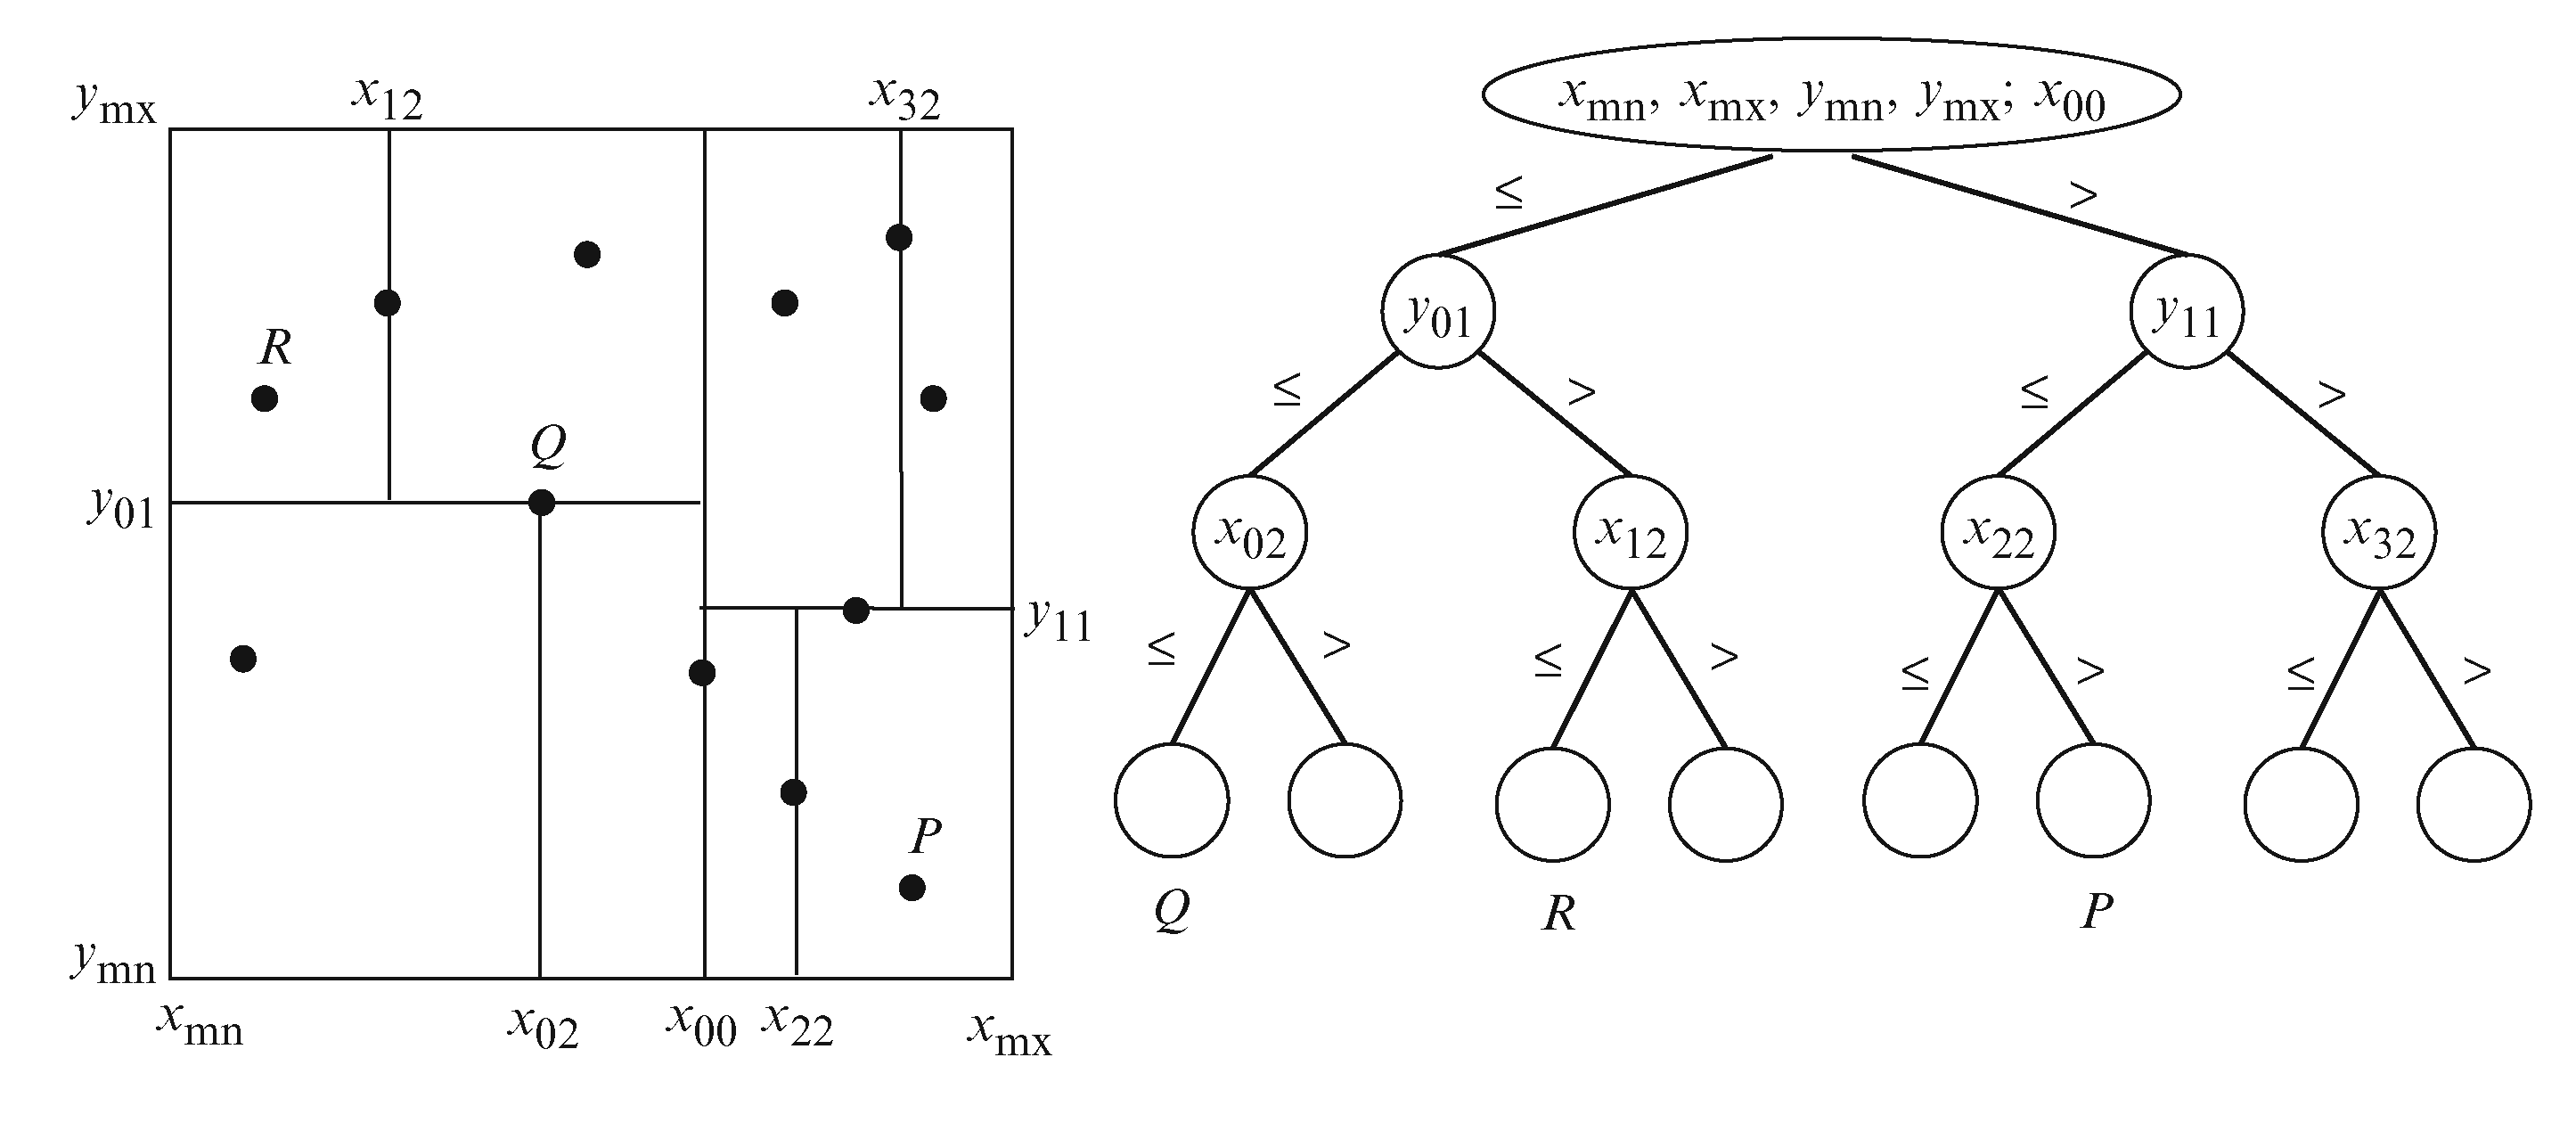
\includegraphics[width=0.9\textwidth]{Img/KD-Tree.png}
\caption{Estructura KD-Tree}
\end{figure}

\end{enumerate}

\section{Implementación}

  Se desarrolló la estructura KDTree implementando los cambios solicitados en la práctica, los cuales se pueden encontrar en el siguiente repositorio Github \href{https://github.com/nestorcal/kdtree}{Estructura KD-Tree}, y se obtienen las siguientes imágenes.


\section{Resultados}

    \begin{enumerate}
    
        \item \textbf{Estructura KD-Tree}

\begin{itemize}
   \item Crear un archivo main.html
\end{itemize}

\begin{figure}[H]
\centering
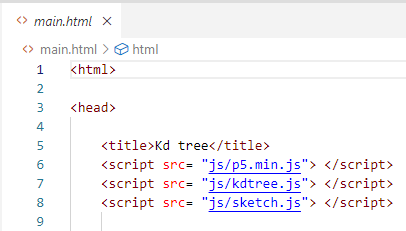
\includegraphics[width=0.9\textwidth]{Img/main.html.png}
\caption{Archivo main.html}
\end{figure}

\begin{itemize}
   \item Crear un archivo kdtree.js
\end{itemize}

\begin{figure}[H]
\centering
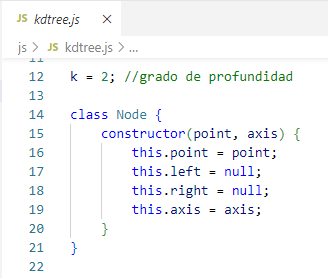
\includegraphics[width=0.4\textwidth]{Img/kdtree.js.png}
\caption{Archivo kdtree.js}
\end{figure}

\begin{itemize}
   \item Construir function getHeight(node) en kdtree.js
\end{itemize}

\begin{figure}[H]
\centering
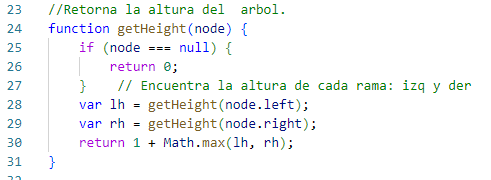
\includegraphics[width=0.7\textwidth]{Img/getHeight_kdtree.png}
\caption{function getHeight(node)}
\end{figure}

\begin{itemize}
   \item Construir function generate dot(node) en kdtree.js
\end{itemize}

\begin{figure}[H]
\centering
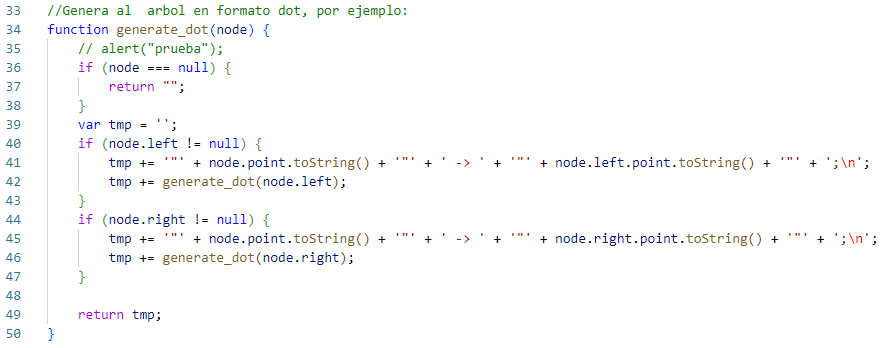
\includegraphics[width=0.9\textwidth]{Img/generate_dot_kdtree.png}
\caption{function generate dot(node)}
\end{figure}

\begin{itemize}
   \item Construir function build kdtree en kdtree.js
\end{itemize}

\begin{figure}[H]
\centering
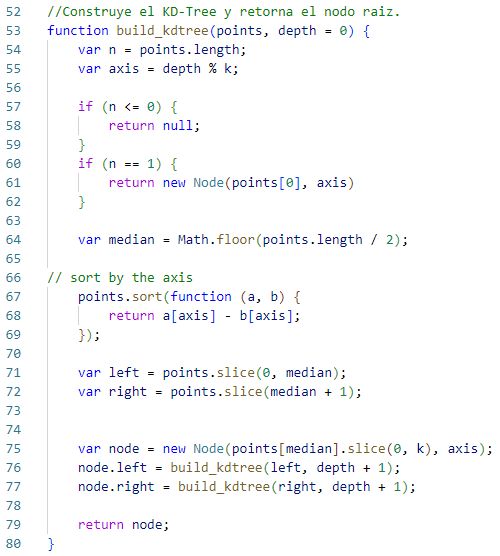
\includegraphics[width=0.6\textwidth]{Img/build_kdtree.png}
\caption{function build kdtree}
\end{figure}

\begin{itemize}
   \item Crear un archivo sketch.js
\end{itemize}

\begin{figure}[H]
\centering
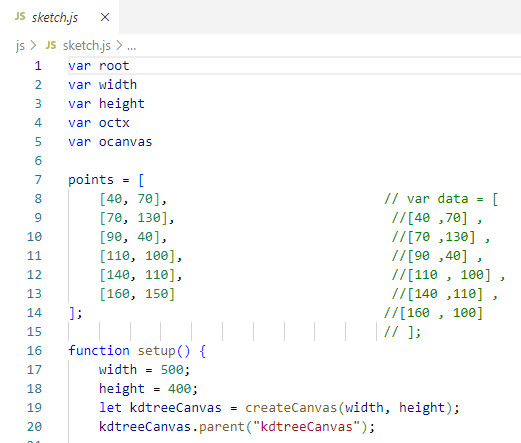
\includegraphics[width=0.56\textwidth]{Img/sketch.js.png}
\caption{Archivo sketch.js}
\end{figure}

\begin{itemize}
   \item Digraph G
\end{itemize}

\begin{figure}[H]
\centering
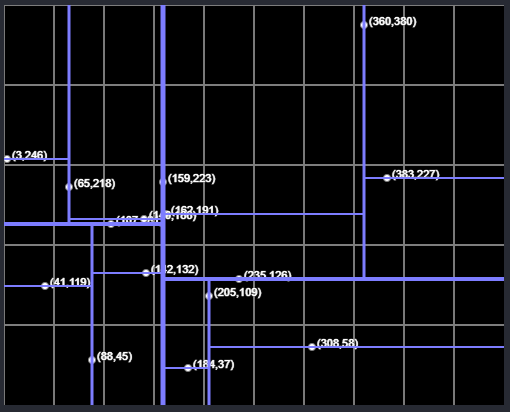
\includegraphics[width=0.56\textwidth]{Img/KD-Tree_example_A.png}
\caption{KD-Tree ejemplo}
\end{figure}

\begin{figure}[H]
\centering
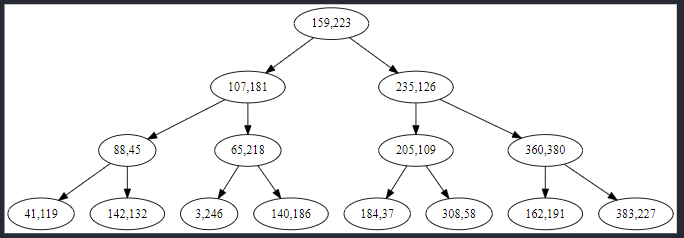
\includegraphics[width=0.56\textwidth]{Img/KD-Tree_example_B.png}
\caption{KD-Tree ejemplo}
\end{figure}

\begin{figure}[H]
\centering
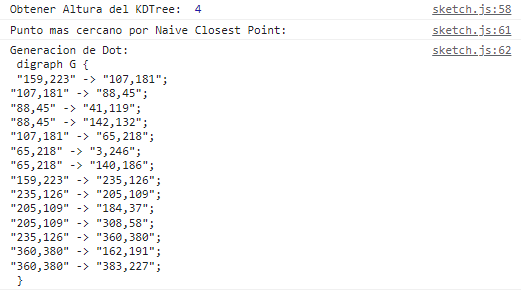
\includegraphics[width=0.7\textwidth]{Img/Digraph G.png}
\caption{KD-Tree ejemplo}
\end{figure}

\begin{itemize}
   \item Implemente la función closest point brute force 
\end{itemize}

\begin{figure}[H]
\centering
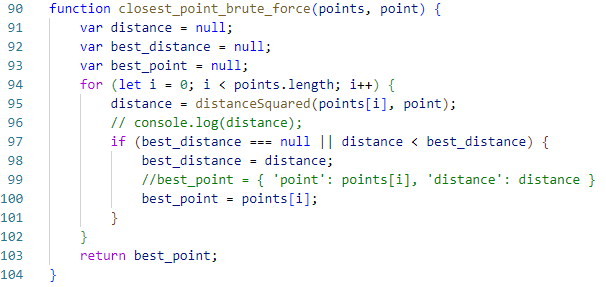
\includegraphics[width=0.9\textwidth]{Img/closest_point_brute_force.png}
\caption{función closest point brute force}
\end{figure}

\begin{itemize}
   \item Implemente la función naive closest point  
\end{itemize}

\begin{figure}[H]
\centering
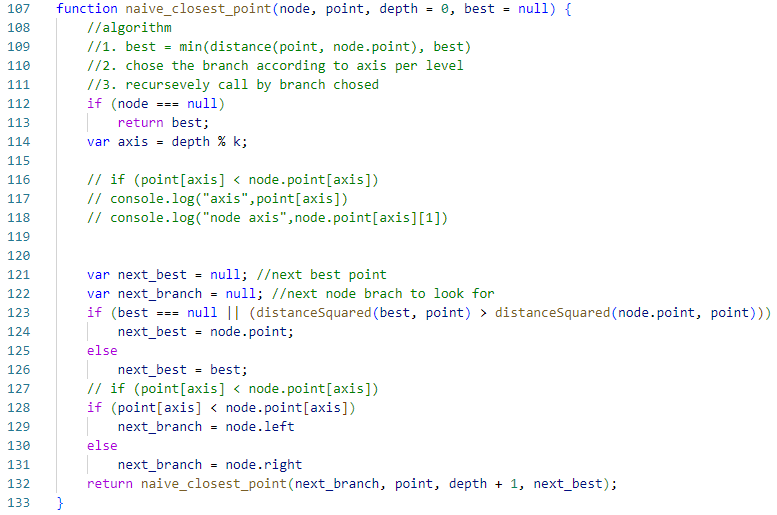
\includegraphics[width=1\textwidth]{Img/naive_closest_point.png}
\caption{función naive closest point}
\end{figure}

\begin{itemize}
   \item value el resultado de las dos funciones implementadas anteriormente con este conjunto de datos: [40,70], [70 ,130], [90,40], [110, 100], [140 ,110], [160, 100]
\end{itemize}

\begin{figure}[H]
\centering
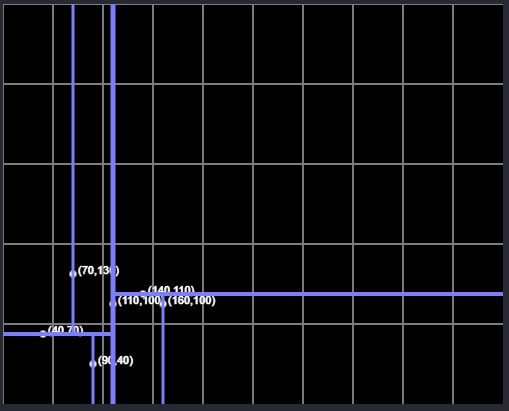
\includegraphics[width=0.67\textwidth]{Img/prueba1.1.png}
\caption{Visualización KD-Tree}
\end{figure}

\begin{figure}[H]
\centering
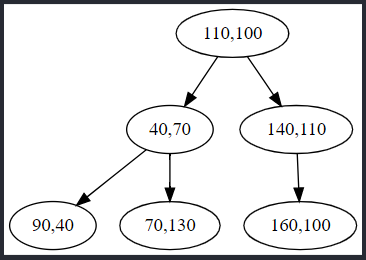
\includegraphics[width=0.4\textwidth]{Img/prueba1.2.png}
\caption{Visualización KD-Tree}
\end{figure}

\begin{figure}[H]
\centering
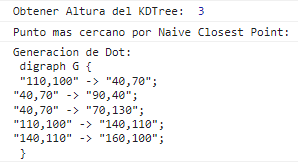
\includegraphics[width=0.4\textwidth]{Img/prueba1.3.png}
\caption{Visualización de la Consola del Navegador}
\end{figure}

\begin{itemize}
   \item value el resultado de las dos funciones implementadas anteriormente con este conjunto de datos: [40,70], [70 ,130], [90,40], [110, 100], [140 ,110], [160, 100] [150, 30]
\end{itemize}

\begin{figure}[H]
\centering
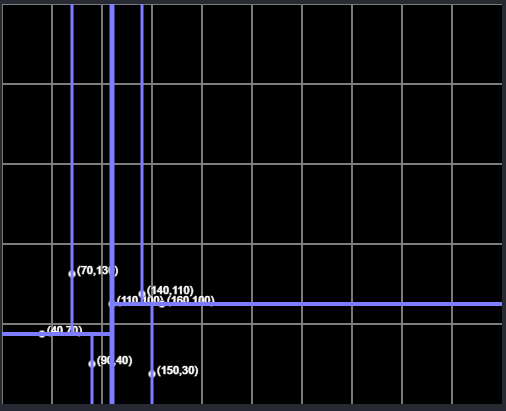
\includegraphics[width=0.7\textwidth]{Img/prueba2.1.png}
\caption{Visualización KD-Tree}
\end{figure}

\begin{figure}[H]
\centering
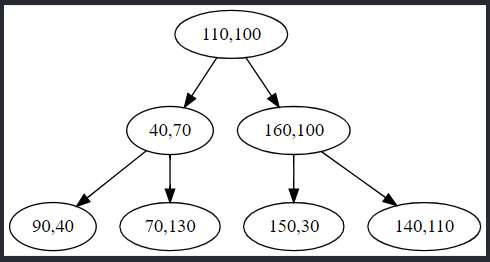
\includegraphics[width=0.4\textwidth]{Img/prueba2.2.png}
\caption{Visualización KD-Tree}
\end{figure}

\begin{figure}[H]
\centering
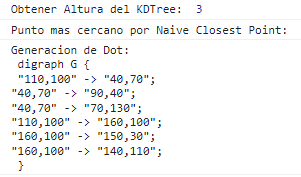
\includegraphics[width=0.4\textwidth]{Img/prueba2.3.png}
\caption{Visualización de la Consola del Navegador}
\end{figure}

\begin{itemize}
   \item Implemente la función closest point
\end{itemize}

\begin{figure}[H]
\centering
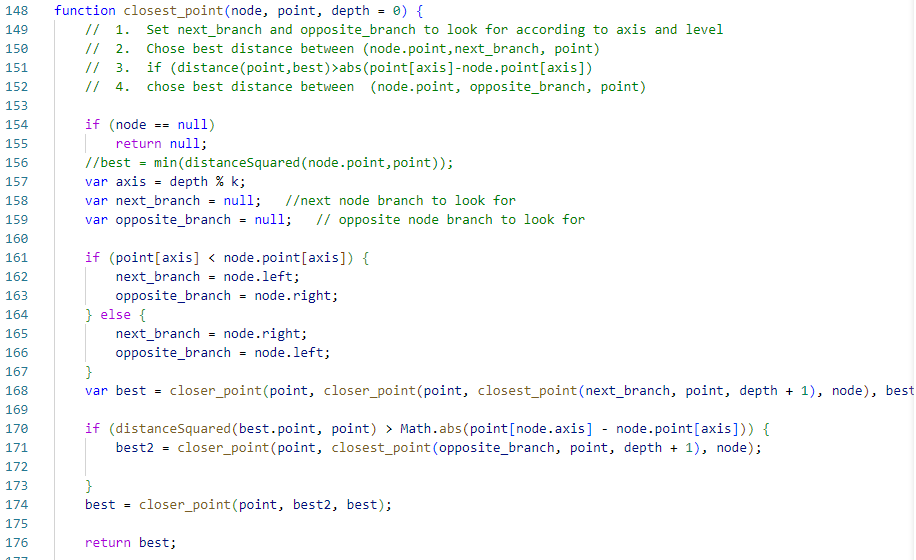
\includegraphics[width=1\textwidth]{Img/closest_point.png}
\caption{función closest point}
\end{figure}

\begin{itemize}
   \item Implemente la función KNN
\end{itemize}

\begin{figure}[H]
\centering
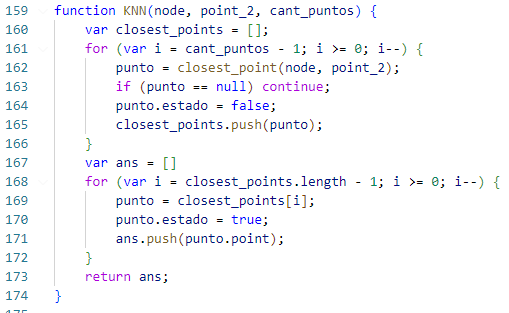
\includegraphics[width=0.8\textwidth]{Img/KNN_kdtree.png}
\caption{función KNN}
\end{figure}

\begin{figure}[H]
\centering
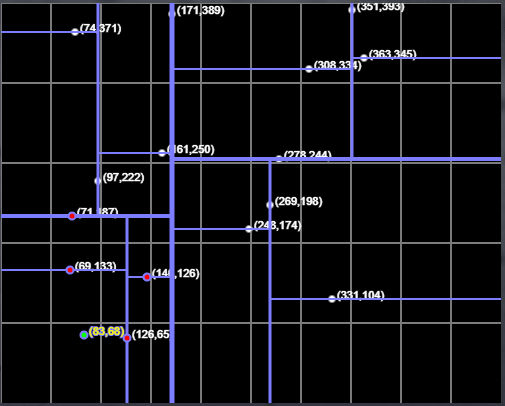
\includegraphics[width=0.7\textwidth]{Img/KNN_kdtree_ej.png}
\caption{función KNN ejemplo}
\end{figure}

\begin{itemize}
   \item Implemente la función range query circle
\end{itemize}

\begin{figure}[H]
\centering
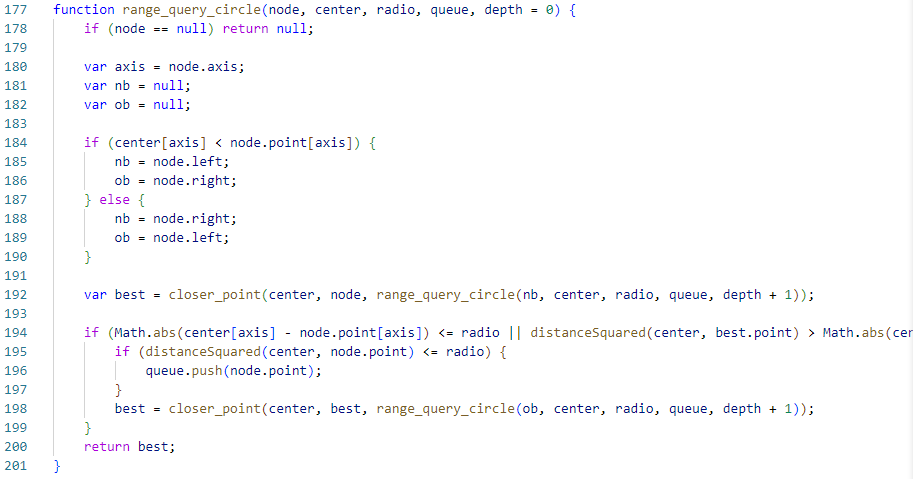
\includegraphics[width=1.1\textwidth]{Img/range_circle.png}
\caption{función range query circle}
\end{figure}

\begin{figure}[H]
\centering
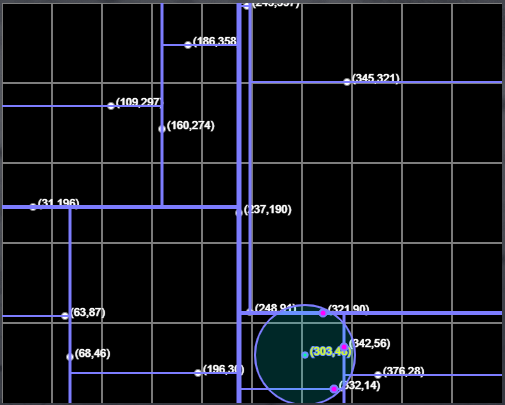
\includegraphics[width=0.8\textwidth]{Img/range_circle_ej.png}
\caption{función range query circle ejemplo}
\end{figure}

\begin{itemize}
   \item Implemente la función range query rec
\end{itemize}

\begin{figure}[H]
\centering
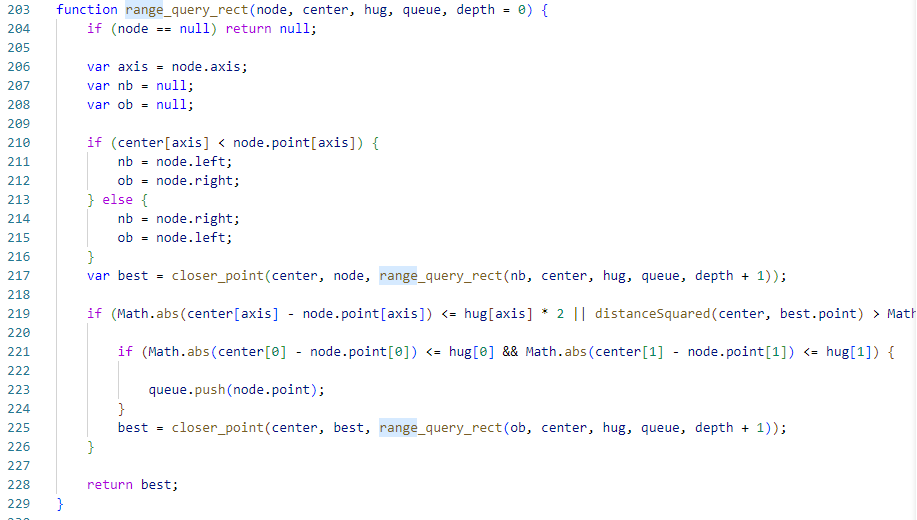
\includegraphics[width=0.9\textwidth]{Img/range_rect.png}
\caption{función range query rec}
\end{figure}

\begin{figure}[H]
\centering
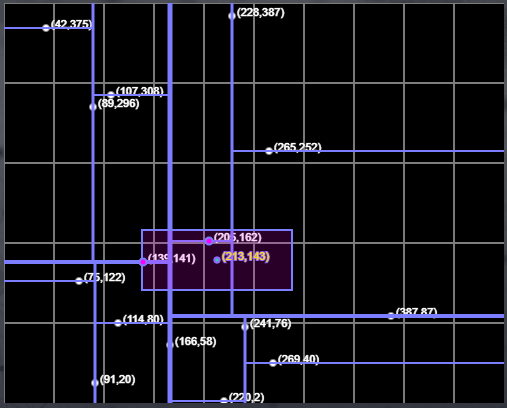
\includegraphics[width=0.8\textwidth]{Img/range_rect_ej.png}
\caption{función range query rec ejemplo}
\end{figure}

\section{Conclusiones}

\begin{itemize}
   \item Se comprueba que mediante la implementación del Kdtree como estructura multidimensional, reduce el número de vecinos a buscar, al calcular la distancia del punto objetivo, técnica utilizada en el algoritmo KNN para clasificación en Machine learning.
   \item El rendimiento de la estructura de datos en inversamente proporcional a la cantidad de los datos, y a su vez, la dimensionalidad del árbol, ya que al incrementar los datos y la dimencionalidad, se irá reduciendo el rendimiento, ya que  cuando se vuelve muy denso, puede haber intersecciones indeseadas con vecinos muy cercanos.
   \item La implementación de algoritmo KD-Tree con tecnologías Html5, JavaScript. P5, ha sido muy intuitivo para comprender el comportamiento de datos multidimensional.

\end{itemize}

    

    \end{enumerate}
	
	%\clearpage
	%\bibliographystyle{apalike}
	%\bibliographystyle{IEEEtranN}
	%\bibliography{bibliography}
		
	
\end{document}